\documentclass[a4paper, 12pt]{article}
%\documentclass{book}

% Important Packages:
 \usepackage{amsmath}    % need for subequations
 \usepackage{amsfonts}
 \usepackage{amsthm}
 \usepackage{graphicx}   % need for figures
 \usepackage{verbatim}   % useful for program listings
 \usepackage{tikz,tkz-euclide}
 \usepackage{amssymb}
 
 \usetikzlibrary{calc,patterns,angles,quotes}
\usetkzobj{all}

\def\deg{^{\circ}}
\newcommand\heading[1]{\ \\\large{\textbf{#1}}}
\newcommand\ora[1]{\overrightarrow{#1}}

\def\thm{Th\textsuperscript{\underline{m}}}

%------------------end---preamble--------------------
 
 % Useful macros 
 \def\tcb#1{\color{blue}{#1}}
 \def\tcr#1{\color{red}{#1}}	
 \def\tcg#1{\color{green}{#1}}
 \def\be{\begin{eqnarray}}	 	\def\ee{\end{eqnarray}}
 \def\bea{\begin{eqnarray}}	 	\def\eea{\end{eqnarray}}
 \def\bean{\begin{eqnarray*}}	\def\eean{\end{eqnarray*}}
 
 \def\D{\displaystyle}
 \def\T{\textstyle}
 \def\l{\left}
 \def\r{\right}
 \def\nf{n_{\!f}} % quark flavours
 \def\pa{\partial}
 \def\eg{e.\,g.}
 \def\ie{i.\,e.}

 \def\be{\begin{equation}}
 \def\ee{\end{equation}}
 \def\bea{\begin{eqnarray}}
 \def\eea{\end{eqnarray}}
 \def\bean{\begin{eqnarray*}}
 \def\eean{\end{eqnarray*}}
 \def\gsim{\mathrel{\rlap{\lower0.2em\hbox{$\sim$}}\raise0.2em\hbox{$>$}}}
 \def\ksim{\mathrel{\rlap{\lower0.2em\hbox{$\sim$}}\raise0.2em\hbox{$<$}}}
 \def\kg{\mathrel{\rlap{\lower0.25em\hbox{$>$}}\raise0.25em\hbox{$<$}}}
 
 \def\AA{${\buildrel_{\circ} \over {\mathrm{A}}}$}
 \def\bm#1{\mbox{\boldmath$#1$}}
 \newcommand{\eq}[1]{(\ref{#1})} 
 \def\pd{\partial}
 \def\d{\textrm{d}} 
 \def\T{\textstyle}
 \def\eg{e.\,g.}	% exempli gratia (for the sake of example)
 \def\ie{i.\,e.}	% id est (that is)


 % Page configuration:
 \topmargin -2.0cm
 \oddsidemargin -0.85cm
 \evensidemargin -0.85cm
 \textwidth 18cm
 \textheight 24cm
 
\begin{document}
\begin{center}
\textbf{April Camp 2019 \\ Senior Test 1} \\
\textbf{Solutions}
\end{center}
\vspace{5mm}

\begin{enumerate}

%  2018 shortlist A1
\item[1.]  \textit{Let $\mathbb{Q}_{> 0}$ denote the set of all positive rational numbers. Determine all functions $f: \mathbb{Q}_{> 0} \to \mathbb{Q}_{> 0}$ satisfying
$$
f \left( x^2 f(y)^2\right) = f(x)^2 f(y) $$
for all $x, y \in \mathbb{Q}_{> 0}$.}
\vspace{5mm}

\textbf{Answer:} $f(x) = 1$ for all $x \in \mathbb{Q}_{> 0}$. \\

\textbf{Solution:} Take any $a, b \in \mathbb{Q}_{> 0}$. By substituting $x = f(a)$, $y = b$, and $x = f(b)$, $y = a$ into the given equation, we get
$$ f(f(a))^2 f(b) = f(f(a)^2 f(b)^2 ) = f(f(b))^2 f(a) $$
which yields
$$
\frac{f(f(a))^2}{f(a)} = \frac{f(f(b))^2}{f(b)} \qquad \textrm{ for all } a, b \in \mathbb{Q}_{> 0}
$$
In other words, this shows that there exists a constant $C \in \mathbb{Q}_{> 0}$ such that $f(f(a))^2 = C f(a)$, or
\begin{equation}  \label{a11}
    \left( \frac{f(f(a))}{C}  \right)^2 = \frac{f(a)}{C} \qquad \textrm{ for all } a \in \mathbb{Q}_{> 0}
\end{equation}

Denote by $f^n(x) = f(f(\dots(f(x))\dots))$ the $n$th iteration of $f$. Equality (\ref{a11}) yields
$$
\frac{f(a)}{C} = \left( \frac{f^2(a)}{C}  \right)^2 = \left( \frac{f^3(a)}{C}  \right)^4 = \dots = \left( \frac{f^{n+1}(a)}{C}  \right)^{2^n}
$$
for all positive integer $n$. So, $f(a)/C$ is the $2^n$-th power of a rational number for all positive integer $n$. This is impossible unless $f(a)/C = 1$, since otherwise the exponent of some prime in the prime decomposition of $f(a)/C$ is not divisible by sufficiently large powers of 2. Therefore, $f(a) = C$ for all $a \in \mathbb{Q}_{> 0}$.

Finally, after substituting $f \equiv C$ into the given condition, we get $C = C^3$, whence $C = 1$. So $f(x) \equiv 1$ is the unique function satisfying the given equation.
\qed \\

\textbf{Comment 1.}  There are several variations of the solution above.  For instance, one may start with finding $f(1) = 1$. To do this, let $d = f(1)$. By substituting $x = y = 1$ and $x = d^2$, $y=1$ into the given, we get $f(d^2) = d^3$ and $f(d^6) = f(d^2)^2 \cdot d = d^7$. By substituting now $x = 1$, $y = d^2$ we obtain $f(d^6) = d^2 \cdot d^3 = d^5$. Therefore, $d^7 = f(d^6) = d^5$, whence $d = 1$.

After that, the rest of the solution simplifies a bit, since we already know that $C = \frac{f(f(1))^2}{f(1)} = 1$. Hence equation (\ref{a11}) becomes merely $f(f(a))^2 = f(a)$, which yields $f(a) = 1$ in a similar manner. \\

\textbf{Comment 2} There exist nonconstant functions $f : \mathbb{R}^+ \to \mathbb{R}^+$ satisfying the given equation for all real $x, y > 0$, for example $f(x) = \sqrt(x)$. \\

\vspace{5mm}
\item[2.]  \textit{Let $n > 1$ be a positive integer. Each cell of an $n \times n$ table contains an integer. Suppose that the following conditions are satisfied:}

\begin{enumerate}
    \item[(i)] \textit{Each number in the table is congruent to $1$ modulo $n$;}
    
    \item[(ii)] \textit{The sum of numbers in any row, as well as the sum of numbers in any column is congruent to $n$ modulo $n^2$.}
    
\end{enumerate}

 \textit{Let $R_i$ be the product of the numbers in the $i$-th row, and $C_j$ be the product of the numbers in the $j$-th column. Prove that the sums $R_1 + \dots + R_n$ and $C_1 + \dots + C_n$ are congruent modulo $n^4$.}
 \vspace{5mm}

\textbf{Proof: } Let $A_{i,j}$ be the entry in the $i$th row and the $j$th column; let $P$ be the product of all $n^2$ entries. For convenience, denote $a_{i, j} = A_{i,j}-1$ and $r_i = R_i - 1$. We show that
\begin{equation} \label{n21}
    \sum_{i=1}^n R_i \equiv (n-1) + P \quad (\textrm{mod } n^4).
\end{equation}

Due to symmetry of the problem conditions, the sum of all the $C_j$ is also congruent to $(n-1) + P$ modulo $n^4$, whence the conclusion.

By condition (i), the number $n$ divides $a_{i, j}$ for all $i$ and $j$. So, every product of at least two of the $a_{i,j}$ is divisible by $n^2$, hence
\begin{equation*}
    R_i = \prod_{j=1}^n (1 + a_{i,j}) = 1 + \prod_{j=1}^n a_{i,j} + \sum_{1 \leq j_1 < j_2 \leq n} a_{i, j_1} a_{i, j_2} + \dots \equiv 1 - n + \sum_{j=1}^n A_{i,j} \quad (\textrm{mod } n^2)
\end{equation*}
for every index $i$. Using condition (ii), we obtain $R_i \equiv 1$ (mod $n^2$), and so $n^2 \,|\, r_i$.

Therefore, every product of at least two of the $r_i$ is divisible by $n^4$. Repeating the same argument, we obtain
$$
P = \prod_{i=1}^n R_i = \prod_{i=1}^n (1 + r_i) \equiv 1 + \sum_{i=1}^n r_i \quad (\textrm{mod } n^4)
$$
whence
$$
\sum_{i=1}^n R_i = n + \sum_{i=1}^n r_i \equiv n + (P-1) \quad (\textrm{mod } n^4)
$$
as desired. \qed \\

\textbf{Solution 2}:  We present a more straightforward (though lengthier) way to establish (\ref{n21}). We also use the notation of $a_{i, j}$.

By condition (i), all the $a_{i, j}$ are divisible by $n$. Therefore, we have

\begin{align*}
    P = \prod_{i=1}^n \prod_{j=1}^n (1 + a_{i, j} ) \equiv 1 + \sum_{(i, j)} a_{i, j} &+ \sum_{(i_1, j_1), (i_2, j_2)} a_{(i_1, j_1)} a_{(i_2, j_2)}  \\
    &+ \sum_{(i_1, j_1), (i_2, j_2), (i_3, j_3)} a_{(i_1, j_1)} a_{(i_2, j_2)} a_{(i_3, j_3)} \quad (\textrm{mod } n^4 ),
\end{align*}

where the last two sums are taken over all unordered pairs/triples of \textit{pairwise different} pairs $(i, j)$; such conventions are applied through the solution.

Similarly,
$$
\sum_{i=1}^n R_i = \sum_{i=1}^n \prod_{j=1}^n (1 + a_{i, j}) \equiv n + \sum_i \sum_j a_{i, j} + \sum_i \sum_{j_1, j_2} a_{i, j_1} a_{i, j_2} + \sum_i \sum_{j_1, j_2, j_3} a_{i, j_1} a_{i, j_2} a_{i, j_3} \quad (\textrm{mod } n^4).
$$

Therefore,
\begin{align*}
    P + (n-1) - \sum_i R_i \equiv \sum_{\substack{(i_1, j_1), (i_2, j_2) \\ i_1 \not = i_2 }} a_{i_1, j_1} a_{i_2, j_2} &+ \sum_{\substack{(i_1, j_1), (i_2, j_2), (i_3, j_3) \\ i_1 \not = i_2 \not = i_3 \not = i_1 }} a_{i_1, j_1} a_{i_2, j_2} a_{i_3, j_3} \\
    &+ \sum_{\substack{(i_1, j_1), (i_2, j_2), (i_3, j_3) \\ i_1 \not = i_2  = i_3 }} a_{i_1, j_1} a_{i_2, j_2} a_{i_3, j_3} \quad (\textrm{mod } n^4).
\end{align*}

We show that in fact each of the three sums appearing in the right-hand part of this congruence is divisible by $n^4$; this yields (\ref{n21}). Denote those three sum sums $\Sigma_1$, $\Sigma_2$, and $\Sigma_3$ in order of appearance. Recall that by condition (i) we have
$$
\sum_j a_{i, j} \equiv 0 \quad (\textrm{mod } n^2) \qquad \textrm{for all indices } i
$$
For every two indices $i_1 < i_2$ we have
$$
\sum_{j_1} \sum_{j_2} a_{i_1, j_1}  a_{i_2, j_2} = \left( \sum_{j_1} a_{i_1, j_1}  \right) \cdot \left( \sum_{j_2} a_{i_2, j_2}  \right) \equiv 0 \quad (\textrm{mod } n^4 ),
$$
since each of the two factors is divisible by $n^2$. Summing over all pairs $(i_1, i_2)$ we obtain $n^4 \,|\, \sum_1$.

Similarly, for every three indices $i_1 < i_2 < i_3$ we have
$$
\sum_{j_1} \sum_{j_2} \sum_{j_3} a_{i_1, j_1} a_{i_2, j_2} a_{i_3, j_3} = \left( \sum_{j_1} a_{i_1, j_1}  \right) \cdot \left( \sum_{j_2} a_{i_2, j_2}  \right) \cdot \left( \sum_{j_3} a_{i_3, j_3}  \right)
$$
which is divisible even by $n^6$. Hence $n^4 \,|\, \Sigma_2$.

Finally, for every indices $i_1 \not = i_2 = i_3$ and $j_2 < j_3$, we have

$$
a_{i_2, j_2} \cdot a_{i_2, j_3} \cdot \sum_{j_1} a_{i_1, j_1} \equiv 0 \quad (\textrm{mod } n^4),
$$
since the three factors are divisible by $n$, $n$, and $n^2$, respectively. Summing over all 4-tuples of indicies $(i_1, i_2, j_1, j_2)$ we get $n^4 \,|\, \Sigma_3$. \qed

\vspace{5mm}
\item[3.]  \textit{A point $T$ is chosen inside a triangle $ABC$. Let $A_1$, $B_1$, and $C_1$ be the reflections of $T$ in $BC$, $CA$, and $AB$, respectively. Let $\Omega$ be the circumcircle of the triangle $A_1 B_1 C_1$. The lines $A_1 T$, $B_1 T$, and $C_1 T$ meet $\Omega$ again at $A_2$, $B_2$, and $C_2$, respectively. Prove that the lines $AA_2$, $BB_2$, and $CC_2$ are concurrent on $\Omega$.}
 \vspace{5mm}

\textbf{Proof: } By $\sphericalangle (\ell, n)$ we always mean the directed angle of the lines $\ell$ and $n$, taken modulo $180^\circ$.

Let $CC_2$ meet $\Omega$ again at $K$ (as usual, if $CC_2$ is tangent to $\Omega$, we set $T = C_2$). We show that the line $BB_2$ contains $K$; similarly, $AA_2$ will also pass through $K$. For this purpose, it suffices to prove that
\begin{equation} \label{g41}
    \sphericalangle (C_2C, C_2A_1) = \sphericalangle (B_2 B, B_2A_1)
\end{equation}

By the problem condition, $CB$ and $CA$ are the perpendicular bisectors of $TA_1$ and $TB_1$, respectively. Hence $C$ is the circumcentre of the triangle $A_1 T B_1$. Therefore,
$$
\sphericalangle (CA_1, CB) = \sphericalangle (CB, CT) = \sphericalangle (B_1 A_1, B_1T) = \sphericalangle (B_1 A_1, B_1 B_2).
$$
In circle $\Omega$, we have $\sphericalangle (B_1 A_1, B_1 B_2) = \sphericalangle (C_2 A_1, C_2 B_2)$. Thus,
$$
\sphericalangle(CA_1, CB) = \sphericalangle(B_1 A_1, B_1 B_2) = \sphericalangle(C_2 A_1, C_2 B_2).
$$
Similarly, we get
$$
\sphericalangle (BA_1, BC) = \sphericalangle (C_1 A_1, C_1 C_2) = \sphericalangle (B_2 A_1, B_2 C_2).
$$
The two obtained relations yield that the triangles $A_1 BC$ and $A_1 B_2 C_2$ are similar and equioriented, hence
$$
\frac{A_1 B_2}{A_1 B} = \frac{A_1 C_2}{A_1 C} \quad 
\textrm{ and } \quad 
\sphericalangle(A_1 B, A_1 C) = \sphericalangle (A_1 B_2, A_1 C_2).
$$

The second equality may be rewritten as $\sphericalangle(A_1 B, A_1 B_2) = \sphericalangle (A_1 C, A_1 C_2)$, so the triangles $A_1 B B_2$ and $A_1 C C_2$ are also similar and equioriented. This establishes (\ref{g41}).

\begin{figure}[h]
    \centering
    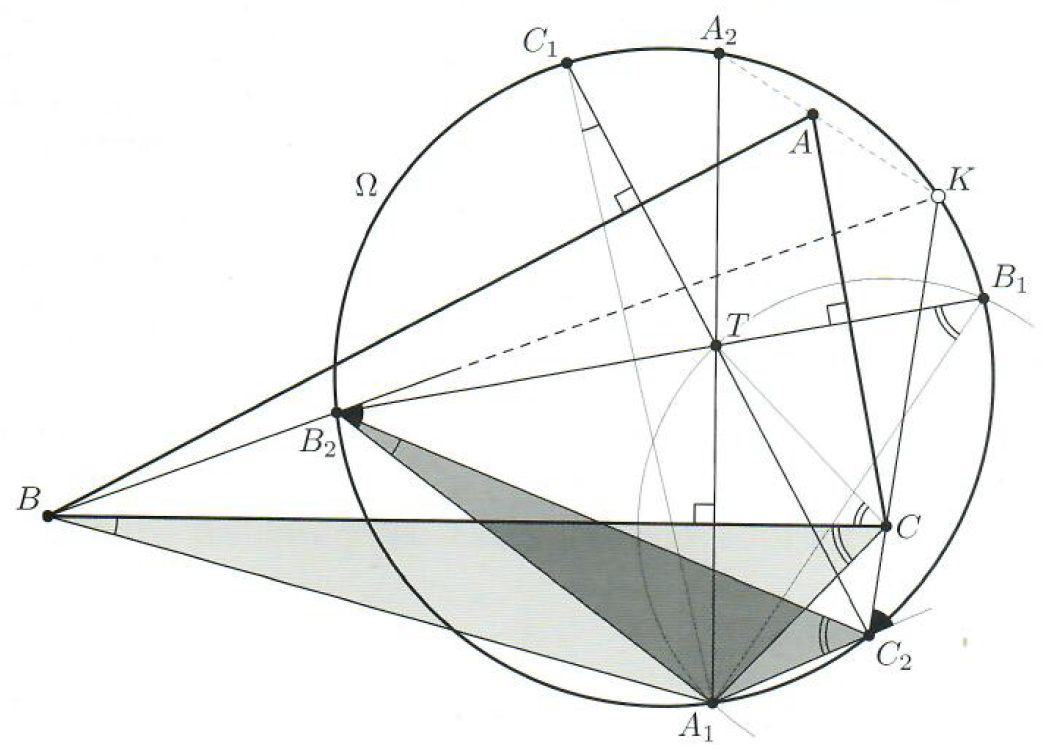
\includegraphics[width = 0.7\textwidth]{2018_G4}
\end{figure}

\textbf{Comment 1}:  In fact, the triangle $A_1 B C$ is an image of $A_1 B_2 C_2$ under a spiral similarity centred at $A_1$; in this case, the triangles $A B B_2$ and $A C C_2$ are also spirally similar with the same centre.

\textbf{Comment 2}:  After obtaining (\ref{g42}) and (\ref{g43}), one can finish the solution in different ways.

For instance, introducing the point $X =  BC \cap B_2 C_2$, one gets from these relations that the 4-tuples $(A_1, B, B_2, X)$ and $(A_1, C, C_2, X)$ are both cyclic. Therefore, $K$ is the Miquel point of the lines $BB_2$, $CC_2$, $BC$, and $B_2 C_2$; this yields that the meeting point of $BB_2$ and $CC_2$ lies on $\Omega$.

Yet another way is to show that the points $A_1, B, C$, and $K$ are concyclic, as
$$
\sphericalangle (KC, KA_1) = \sphericalangle(B_2 C_2, B_2 A_1) = \sphericalangle(BC, BA_1).
$$

By symmetry, the second point $K'$ of intersection of $BB_2$ with $\Omega$ is also concyclic to $A_1, B$, and $C$, hence $K' = K$.

% Diagram 2





\textbf{Comment 3:}  The requirement that the common point of the lines $AA_2$, $BB_2$, and $CC_2$ should lie on $\Omega$ may seem to make the problem easier, since it suggests some approaches.  On the other hand, there are also different ways of showing that the lines $AA_2$, $BB_2$, and $CC_2$ are just concurrent.

In particular, the problem conditions yield that the lines $A_2 T$, $B_2 T$, and $C_2 T$ are perpendicular to the corresponding sides of the triangle $ABC$. One may show that the lines $AT$, $BT$, and $CT$ are also perpendicular to the corresponding sides of the triangle $A_2 B_2 C_2$, i.e. the triangles $ABC$ and $A_2 B_2 C_2$ are \textit{orthologic}, and their orthology centres coincide. It is known that such triangles are also \textit{perspective}, i.e. the lines $AA_2$, $BB_2$, and $CC_2$ are concurrent (in projective sense).

Let $A'$, $B'$ and $C'$ be the projections of $T$ onto the sides of the triangle $ABC$. THen $A_2 T \cdot T A' = B_2 T \cdot TB' = C_2 T \cdot TC'$, since all three products equal (minus) half the power of $T$ with respect to $\Omega$. This means that $A_2$, $B_2$, and $C_2$ are the poles of the sidelines of the triangle $ABC$ with respect to some circle centred at $T$ and having \textit{pure imaginary} radius (in other words, the reflections of $A_2$, $B_2$ and $C_2$ in $T$ are the poles of those sidelines with respect to some regular circle centred at $T$). Hence, dually, the vertices of the triangle $ABC$ are also poles of the sidelines of the triangle $A_2 B_2 C_2$.

\vspace{6mm}


    

\end{enumerate}
\end{document}




